% =====================================================================
%  ch3b_operations.tex — §3.2 A∞ 操作：传播圆盘
% =====================================================================
\subsection{$A_\infty$-操作：传播圆盘}\label{ss:operations}

$\F(M)$ 中的 $A_\infty$-操作由若干（扰动）全纯圆盘的「传播」构形的带权计数决定，其中要用到 $M$ 上某个复结构 $J$（这个选择无关紧要）。为定义
\[
\mu^k:\hom((L_{k-1},\cE_{k-1}),(L_k,\cE_k))\otimes
\dots\otimes \hom((L_0,\cE_0),(L_1,\cE_1))\to
\hom((L_0,\cE_0),(L_k,\cE_k))[2-k],
\]
我们考虑这样的映射：其定义域 $S$ 是一族圆盘的结点并，以一棵带 $k+1$ 个外部边（一个根与 $k$ 个叶）的平面有根树 $T$ 为模型。

对 $T$ 的每个内部顶点 $v_j$，取一个带 $|v_j|$ 个边界标记点的圆盘 $D_j$，并令
\[
S=\Bigl(\bigsqcup_j D_j\Bigr)\Big/\sim,
\]
其中对 $T$ 的每条连接 $v_j,v_{j'}$ 的内部边，把 $D_j$ 与 $D_{j'}$ 在对应于该边两个端点的边界标记点处粘合。所得的结点构形仍带有 $k+1$ 个标记点 $z_0$（对应 $T$ 的根）、$z_1,\dots,z_k$（对应叶），它们沿 $\partial S$ 依此顺序排列。我们把 $\partial S$ 上从 $z_i$ 到 $z_{i+1}$ 的每一段（当 $i=k$ 时是从 $z_k$ 到 $z_0$）标以拉格朗日 $L_i$。

把树 $T$ 从叶到根定向，则 $S$ 的每个分量有一个输出标记点（朝根）与一个或多个输入标记点（朝叶）。我们在这些标记点附近各选带状端，即局部坐标 $s+it$，使输入端以 $\R_+\times[0,1]$ 为模型、输出端以 $\R_-\times[0,1]$ 为模型。再取 $S$ 上的 $1$-形式 $\beta$，使得 $\beta|_{\partial S}=0$，且在每个带状端上 $\beta$ 是 $dt$ 的小正倍数。

\begin{defi}\label{def:proptree}
给定 $L_0,\dots,L_k$、生成元 $p_i\in \cX(L_{i-1},L_i)$（$1\leq i\leq k$）与 $p_0\in \cX(L_0,L_k)$，以及平面树 $T$，\emph{以 $T$ 为模型的传播全纯圆盘}是映射
\[
u:(S,\partial S)\to (M,L_0\cup\dots\cup L_k),
\]
其中定义域 $S$ 以 $T$ 为模型，且满足：
\begin{enumerate}
\item $S$ 的每个分量映到 $M$ 的单个分量；
\item $u$ 在 $S$ 的每个分量上满足扰动 Cauchy--Riemann 方程
\begin{equation}\label{eq:cauchyriemann}
(du-X_h\otimes \beta)^{0,1}=0,
\end{equation}
其中 $h$ 是定义态射空间时所用的正 Hamilton 函数，$\beta$ 是 $S$ 上选定的 $1$-形式；
\item $S$ 的结点映到 $M$ 的节点；
\item $u$ 在每个输入标记点 $z_i$（相应地，输出 $z_0$）处收敛到定义生成元 $p_i\in\cX(L_{i-1},L_i)$（相应地，$p_0\in\cX(L_0,L_k)$）的 $X_{\varepsilon h}$ 流线；
\item 除 $S$ 的结点处、输入标记点 $z_i\in S$ 处，或承载输出标记点 $z_0\in S$ 的常值分量处之外，$u$ 的分量不得穿过 $M$ 的节点；
\item 当输入标记点 $z_i\in S$ 映到 $M$ 的节点时，$u$ 在 $z_i$ 附近带状端上的限制不（在 $M$ 的相应分量中）满射到该节点的邻域上；
\item 若输出标记点 $z_0\in S$ 映到 $M$ 的节点，则 $u$ 在 $S$ 的承载 $z_0$ 的分量上的限制是常值映射。
\end{enumerate}
在固定同伦类 $[u]$ 中、模去重参数化，这类传播圆盘 $u$ 的模空间记为 $\cM(p_0,\dots,p_k,[u])$。
\end{defi}

\begin{figure}[t]
\centering
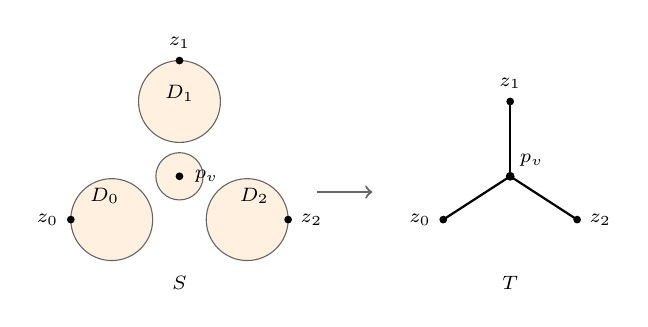
\begin{tikzpicture}[scale=1.0]
% (a) 定义域 S：三个圆盘沿两段内部边粘成
\begin{scope}
  \fill[orange!12,draw=black!60] (0,0.95) circle (0.52);
  \fill[orange!12,draw=black!60] (0.86,-0.55) circle (0.52);
  \fill[orange!12,draw=black!60] (-0.86,-0.55) circle (0.52);
  \fill[orange!12,draw=black!60] (0,0) circle (0.30);
  \fill (0,1.47) circle (1.4pt) node[above=1pt] {\scriptsize $z_1$};
  \fill (1.38,-0.55) circle (1.4pt) node[right=1pt] {\scriptsize $z_2$};
  \fill (-1.38,-0.55) circle (1.4pt) node[left=1pt] {\scriptsize $z_0$};
  \fill (0,0) circle (1.4pt) node[right=2pt] {\scriptsize $p_v$};
  \node at (0,1.05) {\scriptsize $D_1$};
  \node at (0.95,-0.25) {\scriptsize $D_2$};
  \node at (-0.95,-0.25) {\scriptsize $D_0$};
  \node at (0,-1.35) {\scriptsize $S$};
  \draw[->,thick,black!60] (1.75,-0.2)--(2.45,-0.2);
\end{scope}
% (b) 树 T
\begin{scope}[shift={(4.2,0)}]
  \draw[thick,line cap=round] (0,0)--(0,0.95);
  \draw[thick,line cap=round] (0,0)--(0.85,-0.55);
  \draw[thick,line cap=round] (0,0)--(-0.85,-0.55);
  \fill (0,0) circle (1.6pt) node[above right=0pt] {\scriptsize $p_v$};
  \fill (0,0.95) circle (1.4pt) node[above=1pt] {\scriptsize $z_1$};
  \fill (0.85,-0.55) circle (1.4pt) node[right=1pt] {\scriptsize $z_2$};
  \fill (-0.85,-0.55) circle (1.4pt) node[left=1pt] {\scriptsize $z_0$};
  \node at (0,-1.35) {\scriptsize $T$};
\end{scope}
\end{tikzpicture}
\caption{一个对 Floer 乘积 $\mu^2$ 有贡献的传播圆盘（示意图；原书图 3）。左：定义域 $S$，由三个圆盘沿内部边粘成，$p_v$ 为内部节点；右：对应的树 $T$，$z_0$ 为输出端。}\label{fig:proptree_ex}
\end{figure}


（要证明 $A_\infty$-关系所需的粘合行为与一致性，最容易的做法是令 $\beta=\varepsilon\,dt$ 在所有带状端上成立；但在 $M$ 的非紧分量上这未必可行，因为能量估计要求 $d\beta\leq 0$。最简便的绕法是采用 Abouzaid 的重新标定技巧 \cite{AbGen}。另一种做法是对用正 Hamilton 函数 $h$ 的任意小倍数构造的 Floer 复形作局部化，但我们不采用。）

按标准技巧，当 $1$-形式 $\beta$ 闭时，可以把定义在 $S$ 上、边界在 $L_0,\dots,L_k$ 上的扰动全纯曲线 $u$（即 \eqref{eq:cauchyriemann} 的解）改写为真正的全纯曲线 $v:S\to M$（即对某个适当、可能依赖于定义域的复结构的 $(dv)^{0,1}=0$ 的解），其边界在 $L_0^{+k}=\phi_{\varepsilon h}^k(L_0),\dots,L_{k-1}^+=\phi^1_{\varepsilon h}(L_{k-1}),L_k$ 上：只需令
\[
v(z)=\phi_h^{\tau(z)}(u(z)),\qquad d\tau=-\beta.
\]
全纯曲线 $v:S\to M$ 更容易想象与枚举，因为它们就是画在 $M$ 上的多边形，所以我们在作图时（如图~\ref{fig:proptree_ex}）总是采用这一观点。

操作 $\mu^k$ 计数的是\emph{刚性}传播全纯圆盘，即出现在零维模空间中的那些。这恰好发生在每个分量单独刚性的时候，即每个分量都是带局部凸角的浸入多边形。（对承载输出标记点 $z_0$、映到 $M$ 的节点的常值分量，刚性等价于该分量恰有两个输入。）刚性蕴含 Floer 生成元的次数满足
\[
\deg(p_0)=\sum_i \deg(p_i)+2-k .
\]
每个对 $\mu^k$ 有贡献的刚性传播圆盘都带一个权，它由若干与同伦类 $[u]$ 相关的量相乘而得：$u$ 各分量的面积权重与和乐权重（这在 Novikov 域上定义 Fukaya 范畴时是惯例），以及 $S$ 各节点处的\emph{传播系数}——后者是本设定特有的。

考虑 $S$ 的节点 $z_\bullet$，那里一个分量 $D_{in}$ 的输出顶点接到另一分量 $D_{out}$ 的输入顶点上（回忆我们把树 $T$ 从操作的输入即叶，定向到输出即根）。在 $u:S\to M$ 下，$z_\bullet$ 映到 $M$ 的节点 $p_v$，它对应图 $G$ 的某个顶点 $v$；包含 $u(D_{in})$ 与 $u(D_{out})$ 的分量 $M_{e_{in}}$ 与 $M_{e_{out}}$ 在此节点处相接，其中 $e_{in},e_{out}$ 是 $G$ 在 $v$ 处相交的三条边中的两条。由于作为 $u$ 在 $D_{in}$ 与 $D_{out}$ 上边界条件的 $M$ 中的拉格朗日图沿固定方向趋近节点 $p_v$，$u$ 在 $D_{in}$ 与 $D_{out}$ 靠近 $z_\bullet$ 的带状端上的限制具有良定义的整数\emph{次数} $k_{in}$ 与 $k_{out}$，即这些带状端的像在 $M_{e_{in}}$ 与 $M_{e_{out}}$ 内覆盖 $p_v$ 邻域的总重数。例如，图~\ref{fig:proptree_ex} 中构形的两个节点都有 $k_{in}=1$、$k_{out}=0$。一般地，由于 Hamilton 扰动是 $h$ 的小正倍数、且在节点处取局部极小，对非常值映射总有 $k_{in}\geq 1$ 与 $k_{out}\geq 0$。

回忆定义~\ref{def:combidata} 的组合数据包含坐标函数 $t_{e/v}$ 的选取，它在 $x_{e/v}\in X^0_v\simeq\PP^1$ 处为零（对 $G$ 中三条边 $e/v$ 各一个）。函数 $t_{e_{in}/v}^{-k_{in}}$ 在 $x_{e_{in}/v}$ 处有 $k_{in}$ 阶极点，因而可在 $x_{e_{out}/v}$ 的邻域内按 $t_{e_{out}/v}$ 展成幂级数。

\begin{defi}\label{defi:propcoeff}
给定边 $e_{in}/v$、$e_{out}/v$ 与次数 $k_{in}\geq 1$、$k_{out}\geq 0$，\emph{传播系数}
$C^{v;e_{in},e_{out}}_{k_{in},k_{out}}$ 定义为 $t_{e_{in}/v}^{-k_{in}}$ 作为 $t_{e_{out}/v}$ 的幂级数的展开式中 $t_{e_{out}/v}^{k_{out}}$ 的系数。

给定输出不在 $M$ 的节点处的刚性传播圆盘 $u:S\to M$，\emph{传播重数} $\Pi C([u])$ 定义为 $S$ 所有节点处传播系数 $C^{v;e_{in},e_{out}}_{k_{in},k_{out}}$ 之积。
\end{defi}

\begin{example}
回忆我们对 $X^0_v=\PP^1$ 上坐标的优先选取是使它们在三个标记点处取 $0,1,\infty$ 的那些：例如取 $t_0=z$、$t_1=(z-1)/z$、$t_\infty=(1-z)^{-1}$ 作为标记点 $0$、$1$、$\infty$ 附近的坐标。此时
\[
t_0^{-1}=1-t_1=-(t_\infty+t_\infty^2+\dots),
\]
对其他坐标对也类似，于是传播系数为
\[
C^{v;e_{in},e_{out}}_{k_{in},k_{out}}=\begin{cases}
\displaystyle (-1)^{k_{out}}\binom{k_{in}}{k_{out}} & \text{当 }(x_{e_{in}/v},x_{e_{out}/v})\in\{(0,1),(1,\infty),(\infty,0)\},\\[10pt]
\displaystyle (-1)^{k_{in}}\binom{k_{out}-1}{k_{in}-1} & \text{当 }(x_{e_{in}/v},x_{e_{out}/v})\in\{(0,\infty),(1,0),(\infty,1)\}.
\end{cases}
\]
\end{example}

\smallskip
\noindent\textbf{输出映到节点。}
输出标记点 $z_0\in S$ 映到节点 $p_v\in M$ 的情形有所不同。回忆 $S$ 的承载 $z_0$ 的整个分量 $D_0$ 必须映到 $p_v$，而刚性蕴含 $D_0$ 恰有两个输入。若 $D_0$ 的某个输入是 $S$ 的结点，则记 $e_i$ 为 $G$ 的一条边，使得在 $D_0$ 处经该结点接上的 $S$ 的分量映到 $M_{e_i}$；记 $k_i\geq 1$ 为其输出带状端的次数（即进入该节点的次数），并给它配上 $X^0_v\simeq\PP^1$ 上的函数 $t_{e_i/v}^{-k_i}$。若 $D_0$ 的某个输入是 $S$ 的输入标记点，则改取常函数 $1$（相当于令 $k_i=0$）。于是，与常值分量 $D_0$ 相邻的节点对传播重数的贡献，定义为 $t_{e_1/v}^{-k_1}t_{e_2/v}^{-k_2}$ 表成
\[
\{1,\ t_{e_1/v}^{-j},\ t_{e_2/v}^{-j}\ |\ j\geq 1\}
\]
的线性组合时的常数项。这个系数记作 $K^{v;e_1,e_2}_{k_1,k_2}$。（注意：它只能非零当 $S=D_0$（常值曲线对 $\mu^2$ 的贡献），或者 $D_0$ 的两个输入都是 $S$ 的结点且 $e_1\neq e_2$。）传播重数 $\Pi C([u])$ 于是定义为 $K^{v;e_1,e_2}_{k_1,k_2}$（对应与常值分量 $D_0$ 相邻的两个节点）与 $S$ 其他所有节点处传播系数 $C^{v;e_{in},e_{out}}_{k_{in},k_{out}}$ 之积。

\begin{defi}\label{def:areaweight}
边界在 $L_0,\dots,L_k$ 上、输入为 $(p_i,p'_i)\in\cX(L_{i-1},L_i)$、输出为 $(p_0,p'_0)\in\cX(L_0,L_k)$ 的传播全纯圆盘 $u:S\to M$ 的\emph{面积权重}为
\[
W([u]):=T^{A([u])}\,\int_S u^*\mathfrak{b}\in K,\qquad A([u])=\int_S u^*\omega .
\]
当 $L_i$ 配有局部系统 $\cE_i$ 时，$u$ 的\emph{和乐权重}是映射
\begin{align*}
\mathrm{hol}([\partial u]):\bigotimes_{i=1}^k \hom(\cE_{i-1|p_i},\cE_{i|p'_i})&\to \hom(\cE_{0|p_0},\cE_{k|p'_0}),\\
(\rho_1,\dots,\rho_k)&\mapsto \gamma_k\cdot \rho_k\cdot\dots\cdot\gamma_1\cdot\rho_1\cdot\gamma_0,
\end{align*}
其中 $i=0,\dots,k$ 时 $\gamma_i\in\hom(\cE_{i|p'_i},\cE_{i|p_{i+1}})$ 是 $\cE_i$ 的纤维沿 $u(\partial S)$ 位于 $L_i$ 上的那一部分的平行移动所给出的同构。
\end{defi}

为简单起见，且由于本文的主要关注点不在缠绕情形，我们的权用辛面积而不是更常用的\emph{拓扑能量}
\[
E([u])=\int_S u^*\omega-d((u^*h)\,\beta)
\]
来定义。两种概念只相差把每个生成元 $p$ 重新标定为 $T^{\varepsilon h(p)}$，或等价地，在我们的 Hamilton 扰动选取中取极限 $\varepsilon\to 0$；例外是 $M$ 的缠绕非紧端中的生成元。在后一情形，用作用量重新标定更为有利，这样可以完全消去传播圆盘中（只涉及 v.b. 型对象的）缠绕分量的面积贡献。

定义 $\mu^k$ 的最后一个要素是刚性传播圆盘零维模空间的定向。这与黎曼曲面上通常的 Floer 理论完全一样，按 Seidel \cite[\S13]{SeBook} 的处方进行。首先以与上述分次选取一致的方式固定对象的定向，即：点型对象在每个分量中顺时针绕原点，v.b. 型对象在每个分量中从 $0$ 走向 $\infty$。给定输入为 $(p_i,p'_i)\in\cX(L_{i-1},L_i)$、输出为 $(p_0,p'_0)\in\cX(L_0,L_k)$ 的传播圆盘 $u:S\to M$，对每个 $i=0,\dots,k$：若 $\deg p_i$ 为偶，令 $(-1)^{\sigma_i}=+1$；若 $\deg p_i$ 为奇，则当 $L_i$（$i=0$ 时为 $L_k$）在 $p'_i$ 处的定向与定向曲线 $u(\partial S)$ 的定向一致时令 $(-1)^{\sigma_i}=+1$，否则为 $-1$。整体符号为 $(-1)^{\sigma(u)}=\prod_{i=0}^k (-1)^{\sigma_i}$。最后：

\begin{defi}\label{def:mu}
给定 $(p_i,p'_i)\in\cX(L_{i-1},L_i)$ 与 $\rho_i\in\cE_{i-1|p_i}^*\otimes\cE_{i|p'_i}$（$1\leq i\leq k$），令
\[
\mu^k(\rho_k,\dots,\rho_1)=\sum_{\substack{(p_0,p'_0)\in\cX(L_0,L_k)\\ [u]\ \text{刚性}\ u\in\cM(p_0,\dots,p_k,[u])}}
(-1)^{\sigma(u)}\,\Pi C([u])\,W([u])\,\mathrm{hol}([\partial u])(\rho_1,\dots,\rho_k).
\]
\end{defi}
% [Tutor Note: 直觉] 三个权各有分工：面积权重 $W$ 记录圆盘的辛面积（给出 Novikov 变量 $T$ 的指数），和乐权重记录局部系统沿边界的平行移动（给出系数矩阵），传播系数则记录圆盘经过 $M$ 的节点时「坐标 $t_{e/v}$ 的重数如何换算」。前两者是 Fukaya 范畴的常规配方，后者才是本文 A 模型的新增数据。依据：原文 §3.2 与 Def 3.5。
